\section*{External delay optimization}
To produce the analog timing and measure its resolution the parameters of the CFD module needed to be optimized. The thresholds were set to reject events under $\approx$30~keV as show in the calibrated spectra of  Fig.~\ref{fig: calibrated energy spectra}, while the CFD fraction is a fixed value chosen by the producer. The delay, finally, was selected performing test measurements with values in the range 3-6~ns, using the FWHM of timing distribution as resolution indicator as shown in Fig.~\ref{Fig:CFD_Delay}.
\begin{figure}[h!]
	\centering
	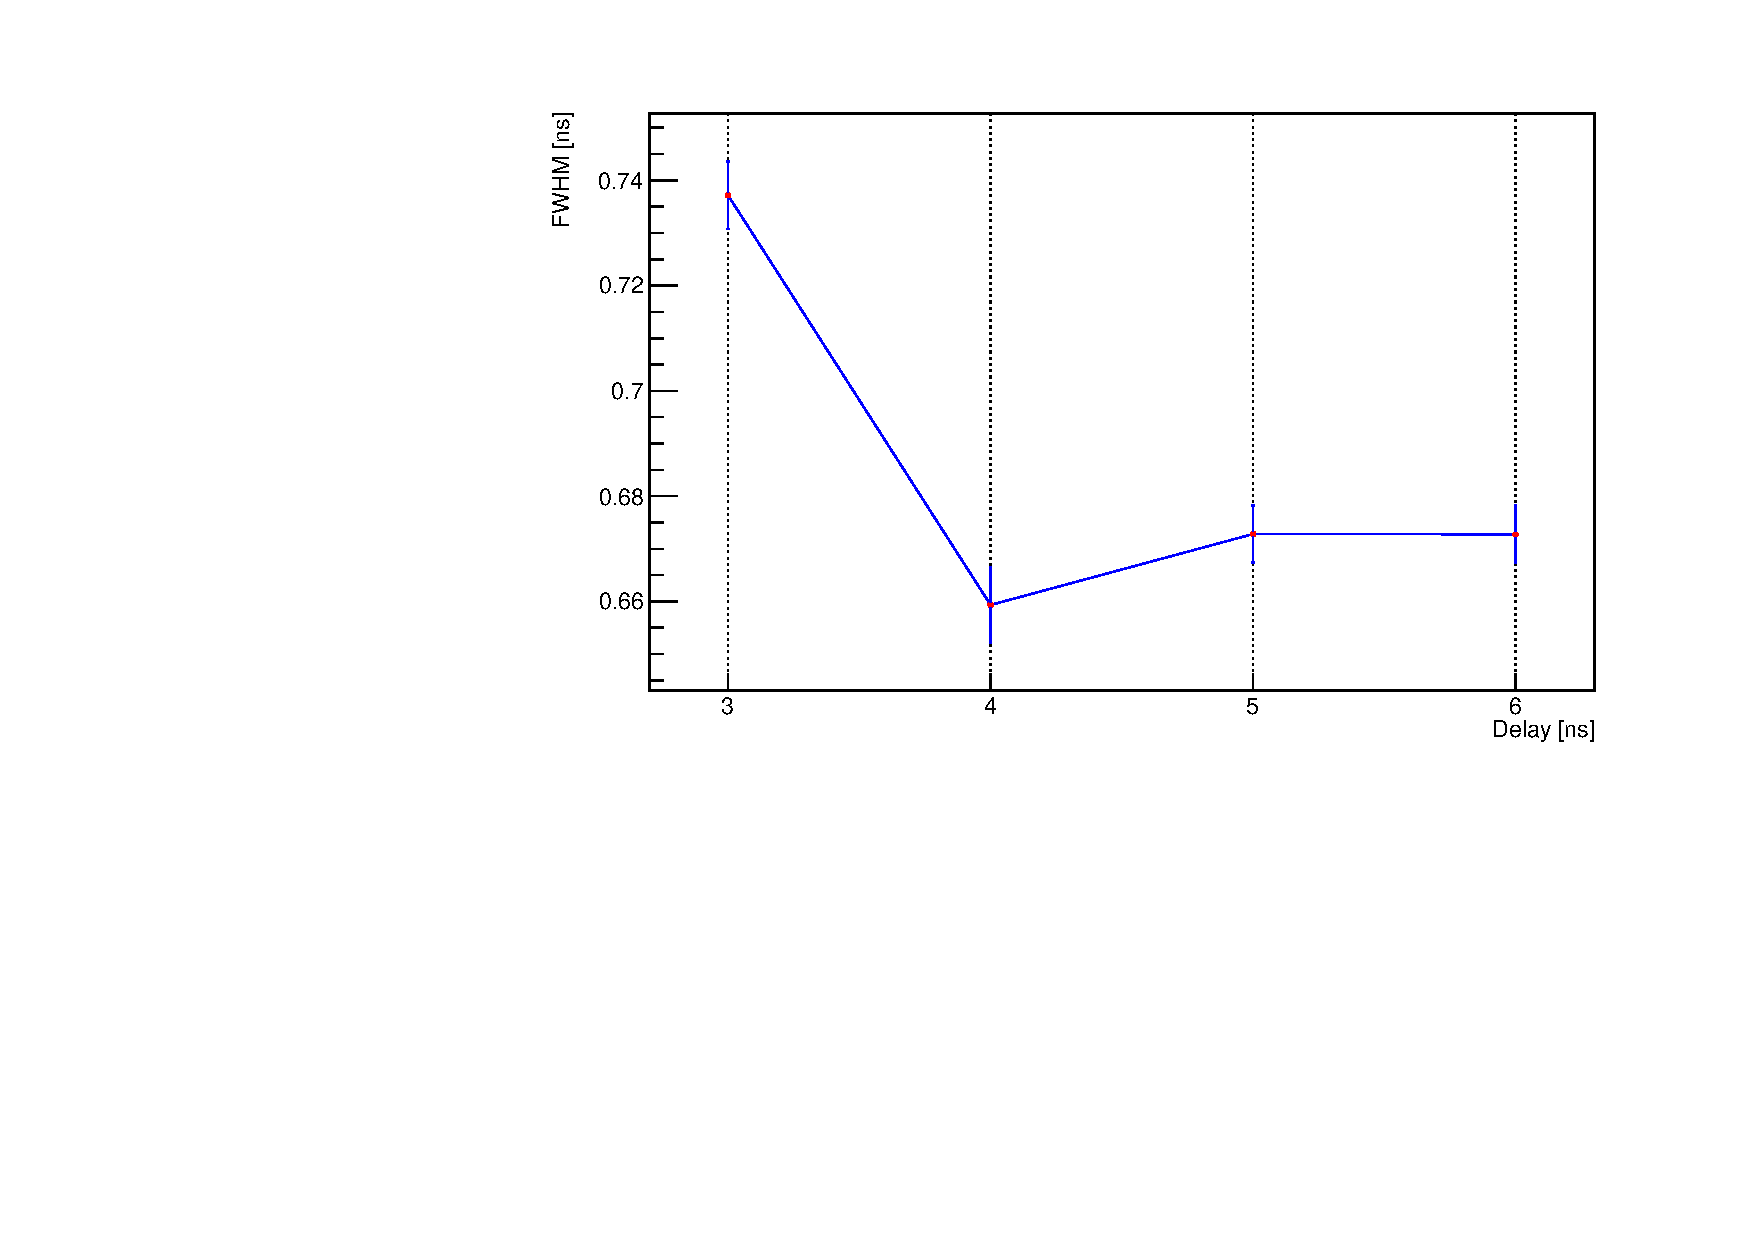
\includegraphics[width = \textwidth]{CFD_del_opt}
	\caption{FWHM as a function of CFD delay.}
	\label{Fig:CFD_Delay}
\end{figure}
\section*{Analog Time resolution as function of energy}
In order to study the time resolution dependence as a function of energy a different radioactive source, $^{60}$Co, was used. This source is chosen because of its high energy Compton Edge ($\approx$1~MeV) that allows to study the energy dependence up to this value. 

Two methods were used to characterize the  timing resolution for different energies: 
\begin{itemize}
	\item Energy Windows
	\item Energy Thresholds
\end{itemize} 
In the following sections they will be described and the obtained results discussed.
\newpage

\subsection*{Energy Windows}
 The analog timing distributions were produced selecting events inside energy windows of 100~keV width in the range 100~keV-1~MeV~(see~Fig.~\ref{Fig:Energy_slice}). 
\begin{figure}[h!]
	\centering
	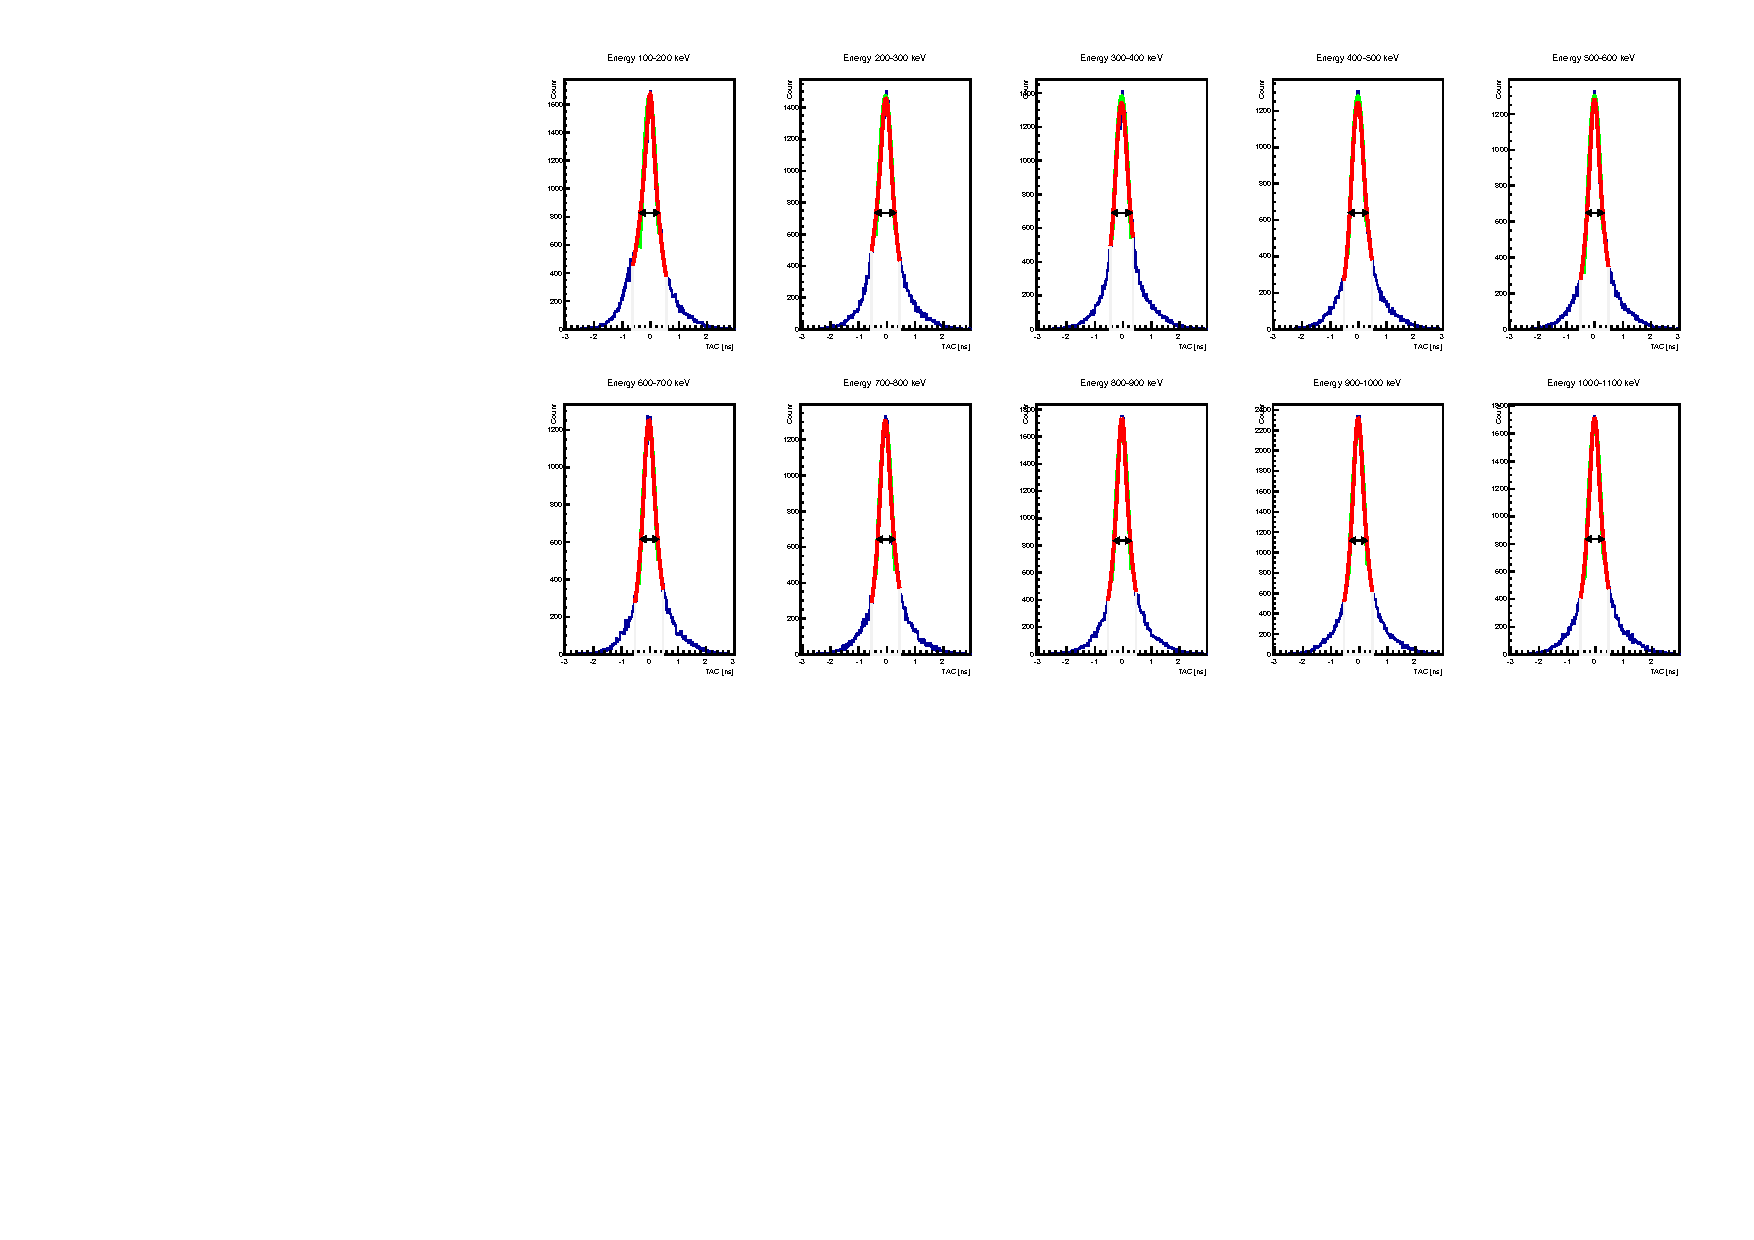
\includegraphics[width = \textwidth]{SlicedTACdists}
	\caption{Timing distributions obtained selecting events inside 100~keV energy windows.}
	\label{Fig:Energy_slice}
\end{figure}

For each distribution the FWHM was computed and reported in the Fig.~\ref{fig: energy windows analog} below, over the 2-D density plot of timing as function of energy.
\begin{figure}[h!]
	\centering
	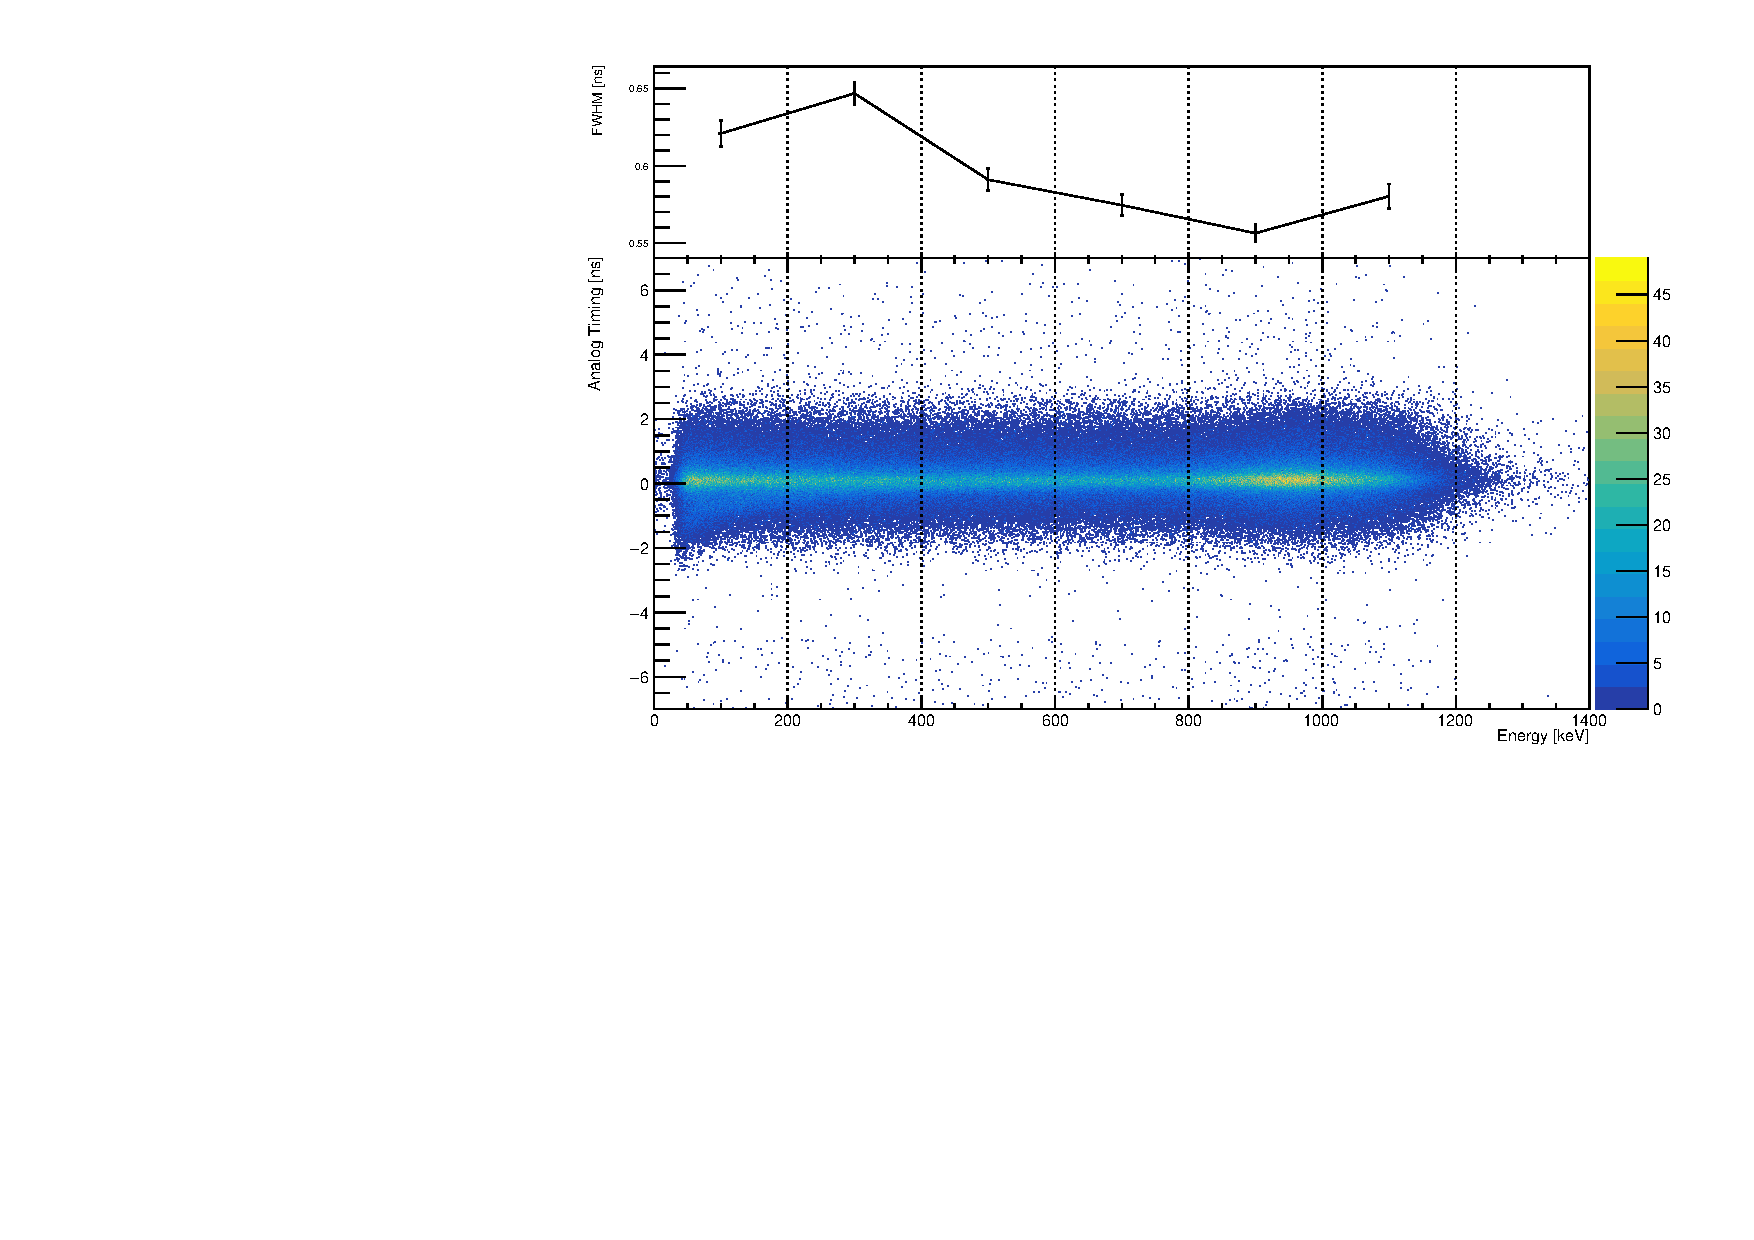
\includegraphics[width = \textwidth]{SlicedTAC_FWHMvs2Ddist}
	\caption{FWHM for each energy slice over 2-D density plot of timing as function of energy. }
	\label{fig: energy windows analog}
\end{figure}

\subsection*{Energy Threshold}
 The analog timing distributions were produced selecting events by mean of different energy thresholds from 100~keV to 1~MeV~(see~Fig.~\ref{Fig: lower energy thr}). 

\begin{figure}[h!]
	\centering
	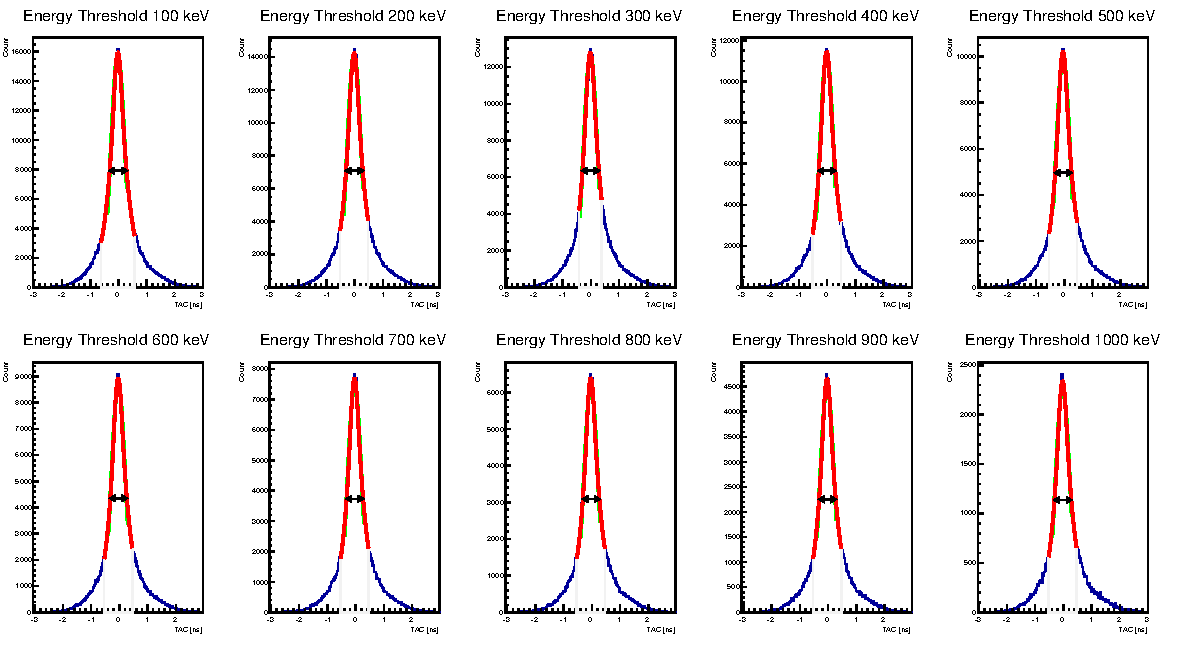
\includegraphics[width = \textwidth]{ThresholdTAC_dists}
	\caption{Timing distributions obtained selecting events by mean of different energy thresholds.}
	\label{Fig: lower energy thr}
\end{figure}

In the same way, for each distribution, the FWHM was computed and reported in the Fig.~\ref{Fig:2Dplot_th} below:

\begin{figure}[h!]
	\centering
	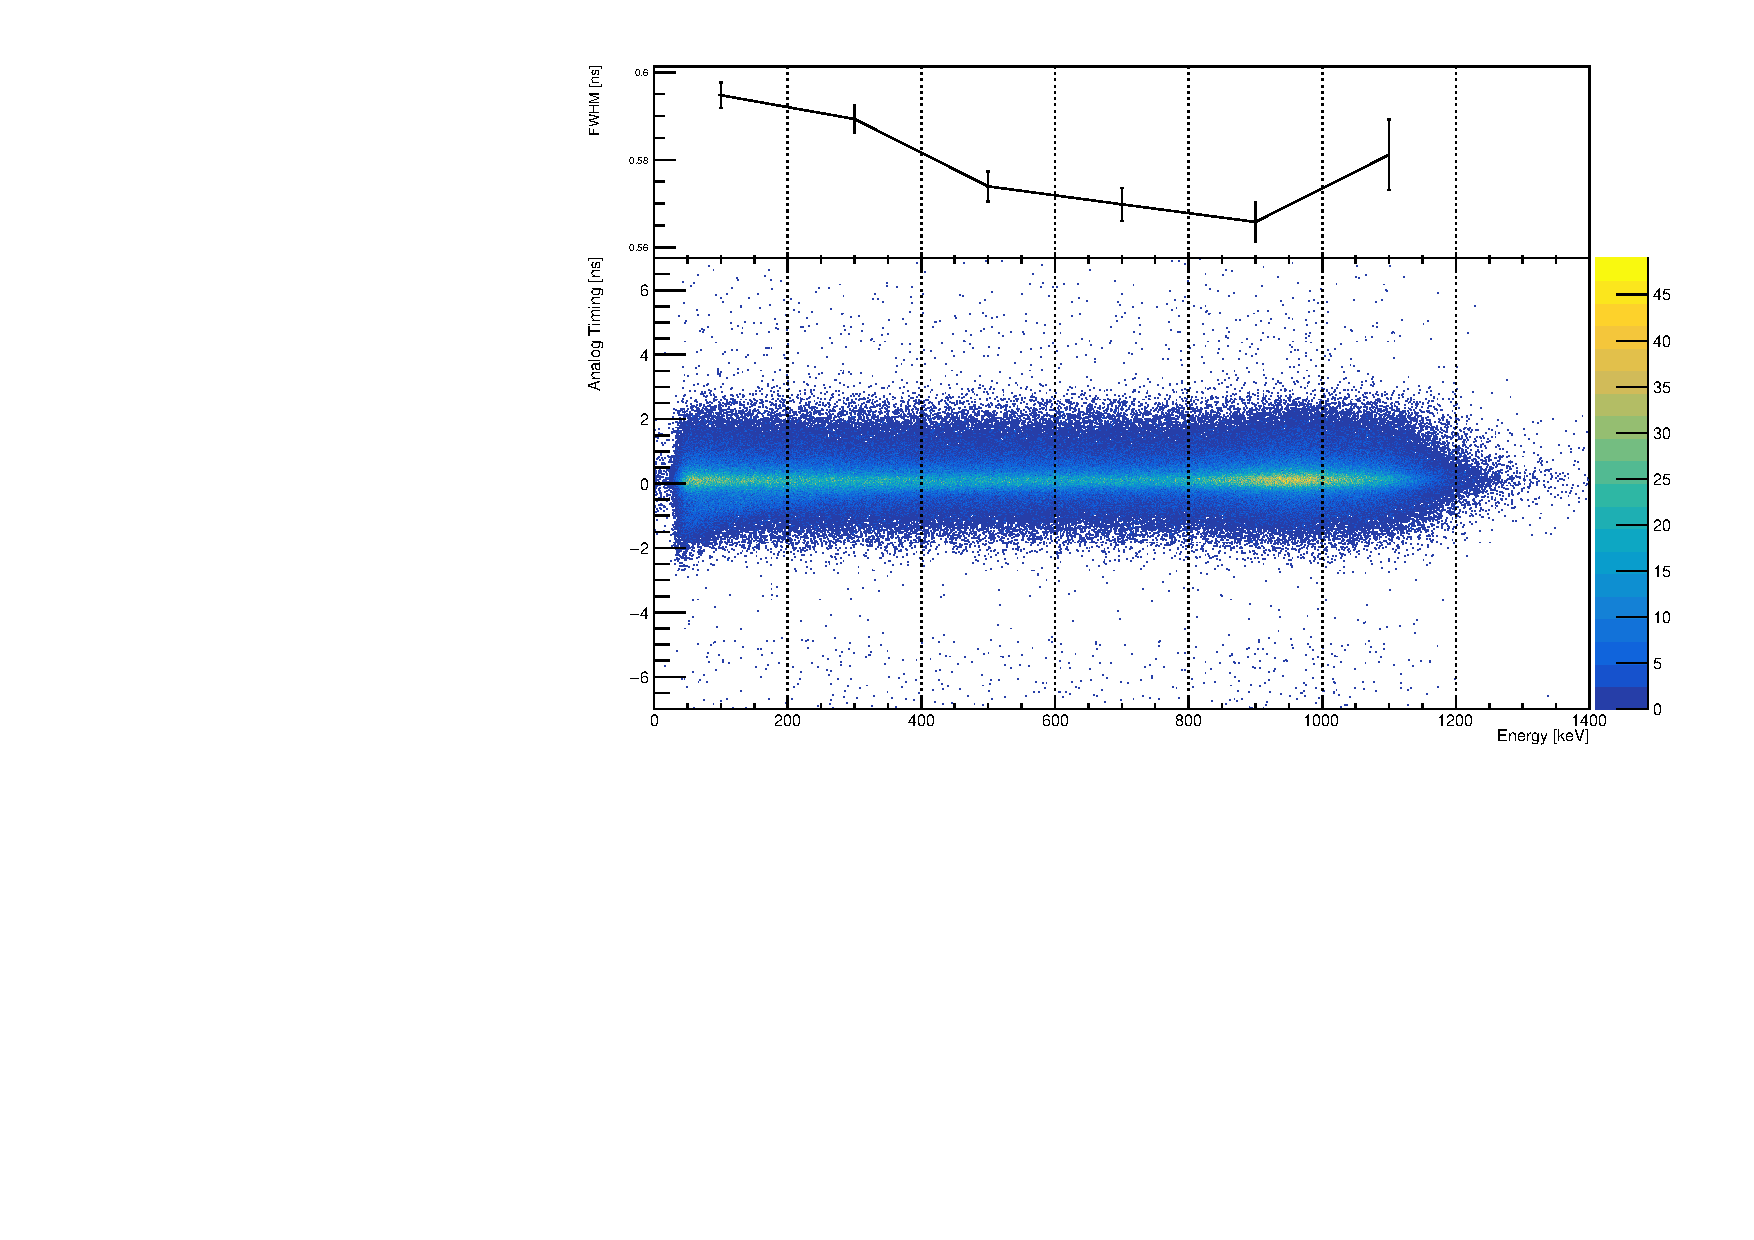
\includegraphics[width = 1\textwidth]{ThresholdTAC_FWHMvs2Ddist}
	\caption{FWHM for each energy threshold over 2-D density plot of timing as function of energy..}
	\label{Fig:2Dplot_th}
\end{figure}

\subsection*{Methods  comparison}

The overlay of the FWHM obtained with the two methods is presented in Fig.~\ref{Fig:Slice_th_comp}. Both the curves show a minimum around the Compton edge of the spectrum, for greater energies the increasing of FWHM could be explained by mean of multi-scattering interactions inside the detectors. 

The worst trend of the energy windows analysis is due by the less statistic of timing distributions with respect to threshold method. This is highlighted observing the FHMW associated errors, which decrease till the Compton edge, were the majority of signals occur. Differently, the opposite trend characterize the thresholds curve, because with increasing energies less events are collected.
\begin{figure}[H]
	\centering
	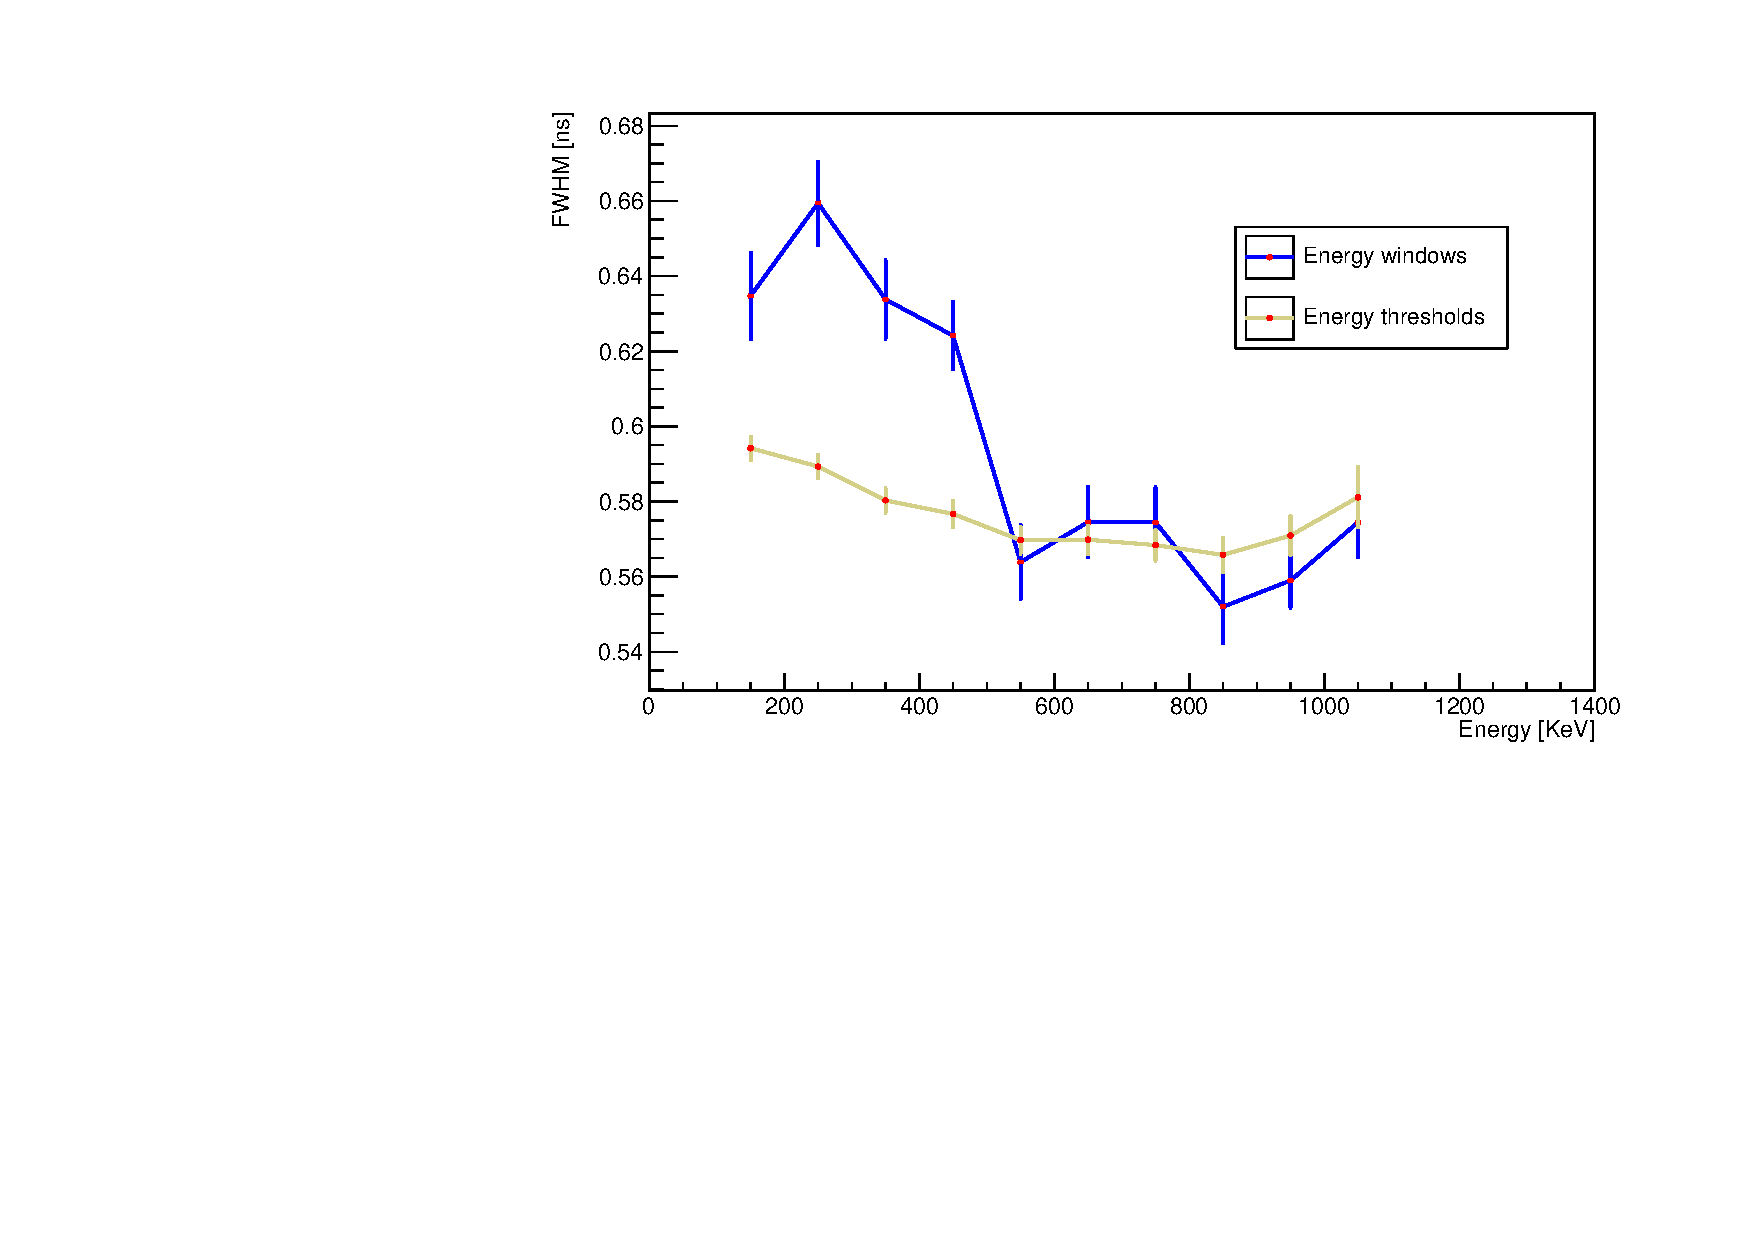
\includegraphics[width = 1\textwidth]{Slice_thresh_comparison}
	\caption{FWHM obtained from different energy windows and different energy thresholds compared.}
	\label{Fig:Slice_th_comp}
\end{figure}










